\documentclass{article}
\usepackage[utf8]{inputenc}
\usepackage{tikz}
\usetikzlibrary{quotes,angles,positioning}

\title{TikZ}
\author{Pontus Vikstål}
\date{April 2019}

\begin{document}

%\maketitle

\newcommand\encircle[1]{%
  \tikz[baseline=(X.base)]
    \node (X) [draw, shape=circle, inner sep=0] {\strut #1};}

\section{Introduction}

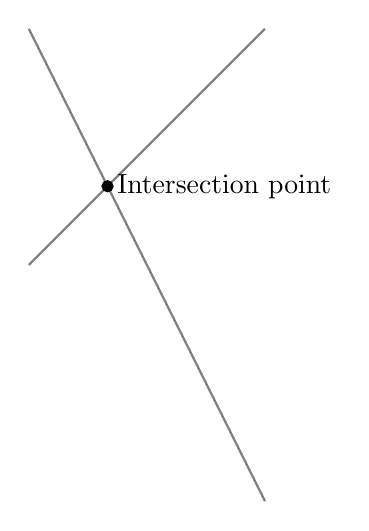
\begin{tikzpicture}
\draw[gray, thick] (-1,2) -- (2,-4);
\draw[gray, thick] (-1,-1) -- (2,2);
\filldraw[black] (0,0) circle (2pt) node[anchor=west] {Intersection point};
\end{tikzpicture}


\begin{tikzpicture}
\draw (-2,0) -- (2,0);
\filldraw [gray] (0,0) circle (2pt);
\draw (-2,-2) .. controls (0,0) .. (2,-2);
\draw (-2,2) .. controls (-1,0) and (1,0) .. (2,2);
\end{tikzpicture}

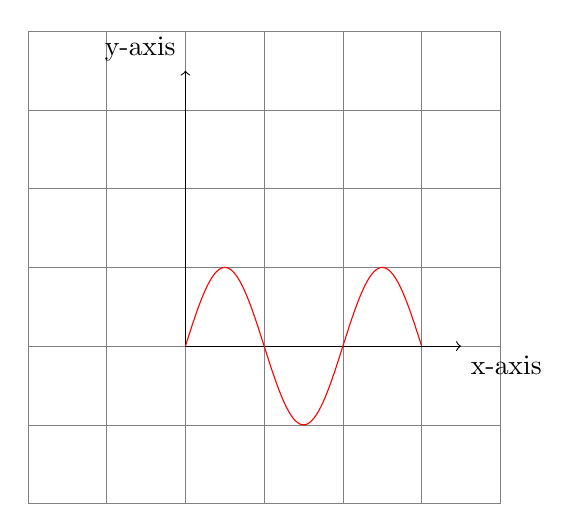
\begin{tikzpicture}
% grid
\draw [help lines] (-2,-2) grid (4,4);
% coordinate system
\draw[->] (0,0) -- (3.5,0) node[anchor=north west] {x-axis};
\draw[->] (0,0) -- (0,3.5) node[anchor=south east] {y-axis};

% draw a sine curve. The trigonometric functions assume that x is in degrees; to express x in radians follow it with the notation "r"
\draw [red, domain=0:3, samples=100] plot (\x, {sin(pi*\x r)});

\end{tikzpicture}

% Bloch sphere
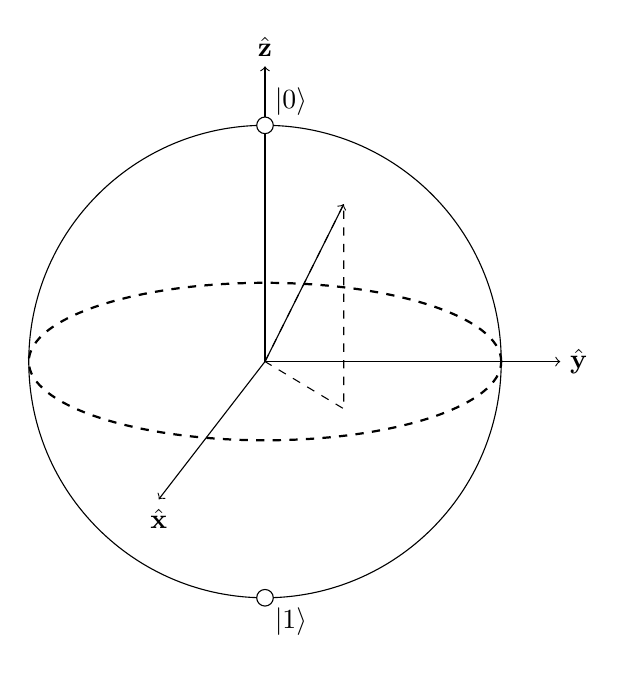
\begin{tikzpicture}[scale=1.5]

  % Define radius
  \def\r{2}

  % Sphere
  \draw (0,0) circle (\r); % circle
  \draw[thick,dashed] (0,0) ellipse (\r{} and \r/3); % ellipse

  % Bloch vector
  \node (orig) at (0,0)          [] {};
  \node (a)    at (\r/3,2*\r/3)  [] {};
  \node (b)    at (\r/3,-\r/5)   [] {};
  %\node [red,above] at (semaphore.north) {$s\le 3$};

  %\draw[] (orig) -- (a) -- (b) -- (orig);
  \draw[->] (0,0) -- (\r/3,2*\r/3);
  \draw[dashed] (0,0) -- (\r/3,2*\r/3) -- (\r/3,-\r/5) -- cycle;


  %\draw (0,0) node[] (orig) {} -- (\r/3,2*\r/3)
  %            node[circle,fill,inner sep=1,label=above:$|\psi\rangle$] (a) {};
  %\draw[dashed] (orig) -- (\r/3,-\r/5) node (phi) {} -- (a);

  % Coordinate system
  \draw[->] (0,0) -- (-\r/5-.5,-\r/3-.5)  node[below] (x1) {$\hat{\mathbf{x}}$};
  \draw[->] (0,0) -- (\r+.5,0)            node[right] (x2) {$\hat{\mathbf{y}}$};
  \draw[->] (0,0) -- (0,\r+.5)            node[above] (x3) {$\hat{\mathbf{z}}$};

  % Angles
  %\pic [draw,angle radius=.5cm,"$\phi$"] {angle = x1--orig--phi};
  %\pic [draw,angle radius=.8cm,"$\theta$"] {angle = a--orig--x3};

  % Computational basis states
  \filldraw[fill=white] (0,2)   circle (2pt) node[anchor=south west] {$|0\rangle$};
  \filldraw[fill=white] (0,-2)  circle (2pt) node[anchor=north west] {$|1\rangle$};

\end{tikzpicture}



\newpage
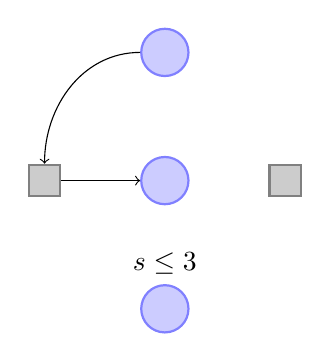
\begin{tikzpicture}
  [place/.style={circle,draw=blue!50,fill=blue!20,thick,
                inner sep=0pt,minimum size=6mm},
  transition/.style={rectangle,draw=black!50,fill=black!20,thick,
                    inner sep=0pt,minimum size=4mm}]
  \node[place]      (waiting)                             {};
  \node[place]      (critical)        [below=of waiting]  {};
  \node[place]      (semaphore)       [below=of critical,
                                      label=above:$s\le3$]{};
  \node[transition] (leave critical)  [right=of critical] {};
  \node[transition] (enter critical)  [left=of critical]  {};

  \draw [->] (enter critical) to (critical);
  \draw [->] (waiting) to [out=180,in=90] (enter critical);

\end{tikzpicture}

\newpage
% Make a circle with a coordiante system, grid lines, sine and cosine, that shows
% pythagoras

\end{document}
